\documentclass[zihao=false,fontset=windows]{ctexart}
% ctexart 不接受任意 pt 选项。正文改 {10pt}，方括号里是行距。
\usepackage{scrextend}
\changefontsizes[12pt]{10pt}

\usepackage[a4paper,left=2.35cm,right=2.35cm,top=1.7cm,bottom=1.9cm]{geometry}
\usepackage{xcolor}
\usepackage{graphicx}
\usepackage{needspace}
\usepackage{amsmath,amssymb}
\usepackage{enumitem}
\usepackage{tabularx}
\usepackage{colortbl}
\usepackage{listings}
\usepackage{hyperref}
\usepackage[most]{tcolorbox}

\definecolor{feishuText}{RGB}{31,35,41}
\definecolor{feishuBlue}{RGB}{36,91,219}
\definecolor{feishuRed}{RGB}{216,57,49}
\definecolor{feishuGray}{RGB}{100,106,115}
\definecolor{feishuGray2}{RGB}{143,149,158}
\definecolor{feishuPinkBg}{RGB}{251,191,188}
\definecolor{quoteBar}{RGB}{51,112,255}
\definecolor{codebg}{RGB}{245,246,247}
\definecolor{codeborder}{RGB}{222,224,227}
\definecolor{inlinebg}{RGB}{242,243,245}
\definecolor{callRed}{RGB}{253,226,226}
\definecolor{callOrange}{RGB}{255,245,235}
\definecolor{callYellow}{RGB}{254,255,240}
\definecolor{callGreen}{RGB}{240,251,239}
\definecolor{callBlue}{RGB}{240,244,255}
\definecolor{callRedSoft}{RGB}{254,241,241}
\definecolor{callSun}{RGB}{255,255,204}
\definecolor{tableHead}{RGB}{242,243,245}
\definecolor{tableRule}{RGB}{222,224,227}
\definecolor{codeText}{RGB}{31,35,41}
\definecolor{codeKeyword}{RGB}{0,0,255}
\definecolor{codeComment}{RGB}{0,128,0}
\definecolor{codeString}{RGB}{163,21,21}

\setmainfont{Times New Roman}
\setCJKmainfont{Microsoft YaHei}[AutoFakeBold=2.2]
\setCJKsansfont{Microsoft YaHei}[AutoFakeBold=2.2]
\setCJKmonofont{Microsoft YaHei}[AutoFakeBold=2.2]
\setmonofont{Consolas}
\newfontfamily\emojifont{Segoe UI Emoji}

\hypersetup{
  colorlinks=true,
  urlcolor=feishuBlue,
  linkcolor=feishuBlue,
  unicode=true,
  pdftitle={SigLIP2}
}

\setlength{\parindent}{0pt}
\setlength{\parskip}{0.42em}
\setlength{\fboxsep}{1.5pt}
\setlength{\emergencystretch}{3em}
\linespread{1.28}
\color{feishuText}
\arrayrulecolor{tableRule}
\urlstyle{same}

\setlist[enumerate]{label=\textcolor{feishuBlue}{\arabic*.}, leftmargin=1.7em, itemsep=0.22em, topsep=0.28em, parsep=0.08em, partopsep=0pt}
\setlist[itemize,1]{label=\textcolor{feishuBlue}{\textbullet}, leftmargin=1.35em, itemsep=0.18em, topsep=0.25em, parsep=0.06em, partopsep=0pt}
\setlist[itemize,2]{label=\textcolor{feishuBlue}{◦}, leftmargin=1.45em, itemsep=0.12em, topsep=0.15em}
\setlist[itemize,3]{label=\textcolor{feishuBlue}{\rule[0.18em]{0.38em}{0.38em}}, leftmargin=1.55em, itemsep=0.1em, topsep=0.12em}

\newcommand{\feiEmoji}[1]{{\emojifont #1}}
\newcommand{\incode}[1]{\colorbox{inlinebg}{\ttfamily\small #1}}
\newcommand{\bigmath}[1]{%
  \begin{center}\large$\displaystyle #1$\end{center}%
}

\lstset{
  language=Python,
  basicstyle=\ttfamily\footnotesize\color{codeText},
  keywordstyle=\color{codeKeyword},
  commentstyle=\color{codeComment},
  stringstyle=\color{codeString},
  showstringspaces=false,
  breaklines=true,
  columns=fullflexible,
  keepspaces=true,
  tabsize=4,
  upquote=true,
  aboveskip=2pt,
  belowskip=0pt,
  xleftmargin=0pt,
  frame=none
}

\tcbset{
  feishubase/.style 2 args={
    enhanced,
    boxrule=0pt,
    arc=8pt,
    left=10pt,
    right=10pt,
    top=7pt,
    bottom=7pt,
    before skip=6pt,
    after skip=6pt,
    colback=#1,
    colframe=#1,
    before upper={\feiEmoji{#2}\hspace{0.45em}\ignorespaces}
  }
}
\newtcolorbox{feishubox}[2]{feishubase={#1}{#2}, breakable}
\newtcolorbox{feishuboxnb}[2]{feishubase={#1}{#2}}

\newtcolorbox{feishuquote}{
  enhanced,
  breakable,
  boxrule=0pt,
  leftrule=3pt,
  arc=0pt,
  colframe=quoteBar,
  colback=white,
  left=8pt,
  right=2pt,
  top=2pt,
  bottom=2pt,
  before skip=4pt,
  after skip=4pt,
  before upper=\color{feishuGray}
}

\newtcolorbox{feishucode}{
  enhanced,
  breakable,
  colback=codebg,
  colframe=codeborder,
  boxrule=0.6pt,
  arc=6pt,
  left=6pt,
  right=6pt,
  top=5pt,
  bottom=4pt,
  before skip=6pt,
  after skip=6pt
}


% 来源：https://scnajei2ds6y.feishu.cn/wiki/H3biwpNrQiAgk2kd9bscXeS2nkb
% fig-03为正常网页截图，密集小字存在截图分辨率限制。
\begin{document}
{\zihao{1}\bfseries SigLIP2\par}
\begin{feishubox}{callOrange}{📒}
论文：《SigLIP 2: Multilingual Vision-Language Encoders with Improved Semantic Understanding, Localization, and Dense Features》\par
论文链接：\href{https://arxiv.org/pdf/2502.14786}{https://arxiv.org/pdf/2502.14786}\par
GitHub：\href{https://link.zhihu.com/?target=https\%3A//github/}{https://github}\href{https://link.zhihu.com/?target=https\%3A//github/}{. com/google-research/big\_vision}\par
\end{feishubox}
\par\vspace{1.15em}\noindent{\zihao{-2}\bfseries \textcolor{feishuBlue}{1.} 背景}\par\vspace{0.28em}
SigLIP2主要改进：\par
\begin{itemize}
\item 训练目标：在SigLIP的图像-文本sigmoid对比损失的基础上，结合了 LocCa 的基于解码器的预训练以及 SILC 和 TIPS 中的自蒸馏和掩码预测任务。\par
\item 隐式蒸馏：并且通过主动样本选择进行隐式蒸馏，提升小型模型的性能。\par
\item 可变分辨率：SigLIP2包含一个 NaFlex 变体，支持多种分辨率并保留图像的原始长宽比。\par
\end{itemize}
通过这些改进，SigLIP 2模型在所有模型规模上的核心能力均优于SigLIP，包括零样本分类、图像-文本检索，以及在提取视觉-语言模型（VLMs）的视觉表示时的迁移性能。\par
\par\vspace{1.15em}\noindent{\zihao{-2}\bfseries \textcolor{feishuBlue}{2.} SigLIP2}\par\vspace{0.28em}
模型架构上还是Image Encoder+Text Encoder的架构，但是训练架构上有三个任务：\par
\par\noindent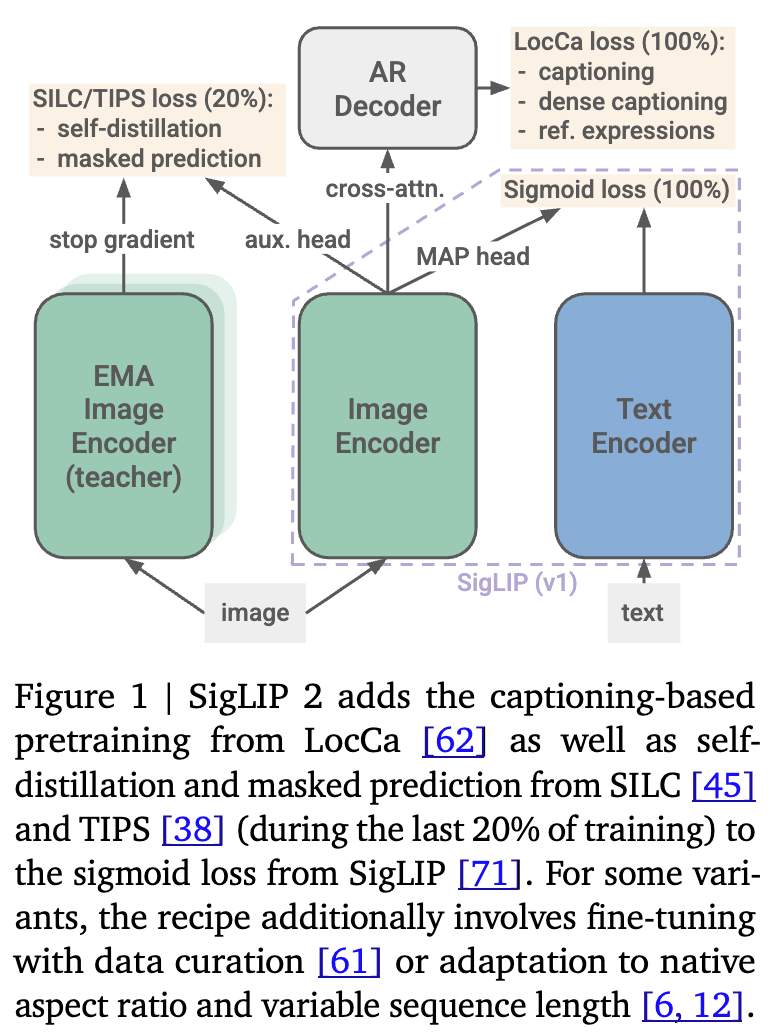
\includegraphics[width=0.43\textwidth]{images/SigLIP2/fig-01.png}\par
\par\vspace{0.95em}\noindent{\zihao{3}\bfseries \textcolor{feishuBlue}{2.1} Sigmoid  Loss}\par\vspace{0.28em}
这一部分和SigLIP是一样的。即SigLIP 通过将每个图像嵌入与小批量中的每个文本嵌入组合，创建二元分类问题，并通过逻辑回归（sigmoid 损失）训练嵌入，以分类匹配和不匹配的对。\par
\par\vspace{0.95em}\noindent{\zihao{3}\bfseries \textcolor{feishuBlue}{2.2} LocCa Loss}\par\vspace{0.28em}
对于 LocCa，在未池化的视觉编码器表示（在应用 MAP 头之前）上附加了一个带有交叉注意力的标准 Transformer 解码器。解码器的结构与文本编码器相似，但增加了交叉注意力层，并将层数减少了一半。除了图像描述生成，LocCa还训练自动指称表达预测和基础描述生成。前者是预测描述特定图像区域的字幕的边界框坐标，而后者是给定边界框坐标预测区域特定的字幕。区域与字幕的配对通过首先从替代文本中提取n-gram，然后使用OWLv2中的方法进行开放词汇检测来自动标注。此外，我们使用PaLI中固定的对象类别集，而不是n-gram。对于每个示例，解码器被训练以预测所有三个目标（相当于三次解码器前向传递）。字幕生成目标以50\%的概率通过并行预测进行预测，即所有字幕标记从掩码标记中并行预测，不使用因果注意力掩码。最后，为了减少由于大词汇量导致的内存消耗，实现分块版本的解码器损失。\par
\par\vspace{0.95em}\noindent{\zihao{3}\bfseries \textcolor{feishuBlue}{2.3} SILC/TIPS Loss}\par\vspace{0.28em}
SILC和TIPS通过自蒸馏和掩码预测损失进行局部到全局的对应学习，以提升（未池化）特征表示的局部语义。这种表示通常用于像分割、深度估计等密集预测任务。\par
第一个项是来自SILC的局部到全局一致性损失，其中视觉编码器作为学生网络，仅获取训练图像的部分（局部）视图，并被训练来匹配从完整图像得出的教师表示。这个辅助匹配任务在一个用单独的MLP头计算的高维特征空间中执行。通常，教师的参数通过对学生参数在之前迭代中的指数移动平均（EMA）获得。我们依赖一个全局（教师）视图和8个局部（学生）视图，其他方面则遵循SILC中的增强、损失和超参数。\par
第二个损失项是来自TIPS的掩码预测目标。我们在学生网络中将50\%的嵌入图像块替换为掩码标记，并训练学生在被掩盖的位置上匹配教师的特征。该损失的定义与第一个项（即一致性损失）相同，但应用于每个图像块的特征，而不是池化的图像级表示。此外，学生和教师都看到相同的全局视图（学生的视图会有掩码处理）。\par
在训练完成的80\%时加入这些损失，将教师的参数初始化为学生的参数，而其余附加参数（如头部、掩码标记及相应的优化器参数）则随机初始化。我们使用原始图像计算上一节中的SigLIP和LocCa损失，并在额外增强的视图上应用附加损失。这样做是为了确保数据增强不会对图像-文本对齐产生负面影响，这也是SILC的建议。第一个和第二个损失项的权重分别设为1和0.25。此外，为了平衡模型在全局/语义和密集任务上的质量，我们对这两个损失项分别按0.25、0.5、1.0和0.5的系数重新加权，适用于B、L、So400m和g模型大小。\par
\par\vspace{0.95em}\noindent{\zihao{3}\bfseries \textcolor{feishuBlue}{2.4} 可变尺寸和分辨率(NaFlex)}\par\vspace{0.28em}
针对多分辨率输入，SigLIP 2 采用了 NaFlex 模型，它结合了不同分辨率和保留图像原生纵横比的思想。该模型在处理图像时，首先调整输入图像的大小，以确保其高度和宽度在调整后是patch大小的倍数，同时尽量减少纵横比的失真 。通过这种方法，可以使用适合不同类型图像的适当分辨率，并在任务中降低失真对性能的影响。\par
此外，NaFlex 支持多种预定义的序列长度，使得模型能够更有效地处理不同的输入类型 。在训练阶段，模型从默认检查点开始，调整训练来适应变化的纵横比和分辨率，从而实现更好的处理和性能。\par
\Needspace{14cm}
\par\vspace{1.15em}\noindent{\zihao{-2}\bfseries \textcolor{feishuBlue}{3.} 实验}\par\vspace{0.28em}
\par\vspace{0.95em}\noindent{\zihao{3}\bfseries \textcolor{feishuBlue}{3.1} 零样本分类和检索}\par\vspace{0.28em}
\begin{tcbraster}[raster columns=100,raster equal height=rows,raster column skip=0pt,raster row skip=8pt,raster left skip=0pt,raster right skip=0pt]
\begin{tcolorbox}[blankest,raster multicolumn=47,right=8pt,valign=top]
SigLIP 2在零样本分类（ImageNet、ObjectNet、ImageNetv2、ImageNet ReaL）和图文检索基准上的性能都优于SigLIP和其他（开放权重）基准。\par
\vspace{1em}
需要注意的是，DFN在这些基准上最接近SigLIP 2，它使用在ImageNet、COCO和Flickr上微调的网络作为过滤器来提高数据质量。\par
\vspace{1em}
由于蒸馏的原因，SigLIP2在B尺寸模型上对基准的改进尤为显著。此外，我们观察到常见的缩放趋势是图像分辨率和模型大小的函数。\par
\end{tcolorbox}
\begin{tcolorbox}[blankest,raster multicolumn=53,left=1pt,valign=top]
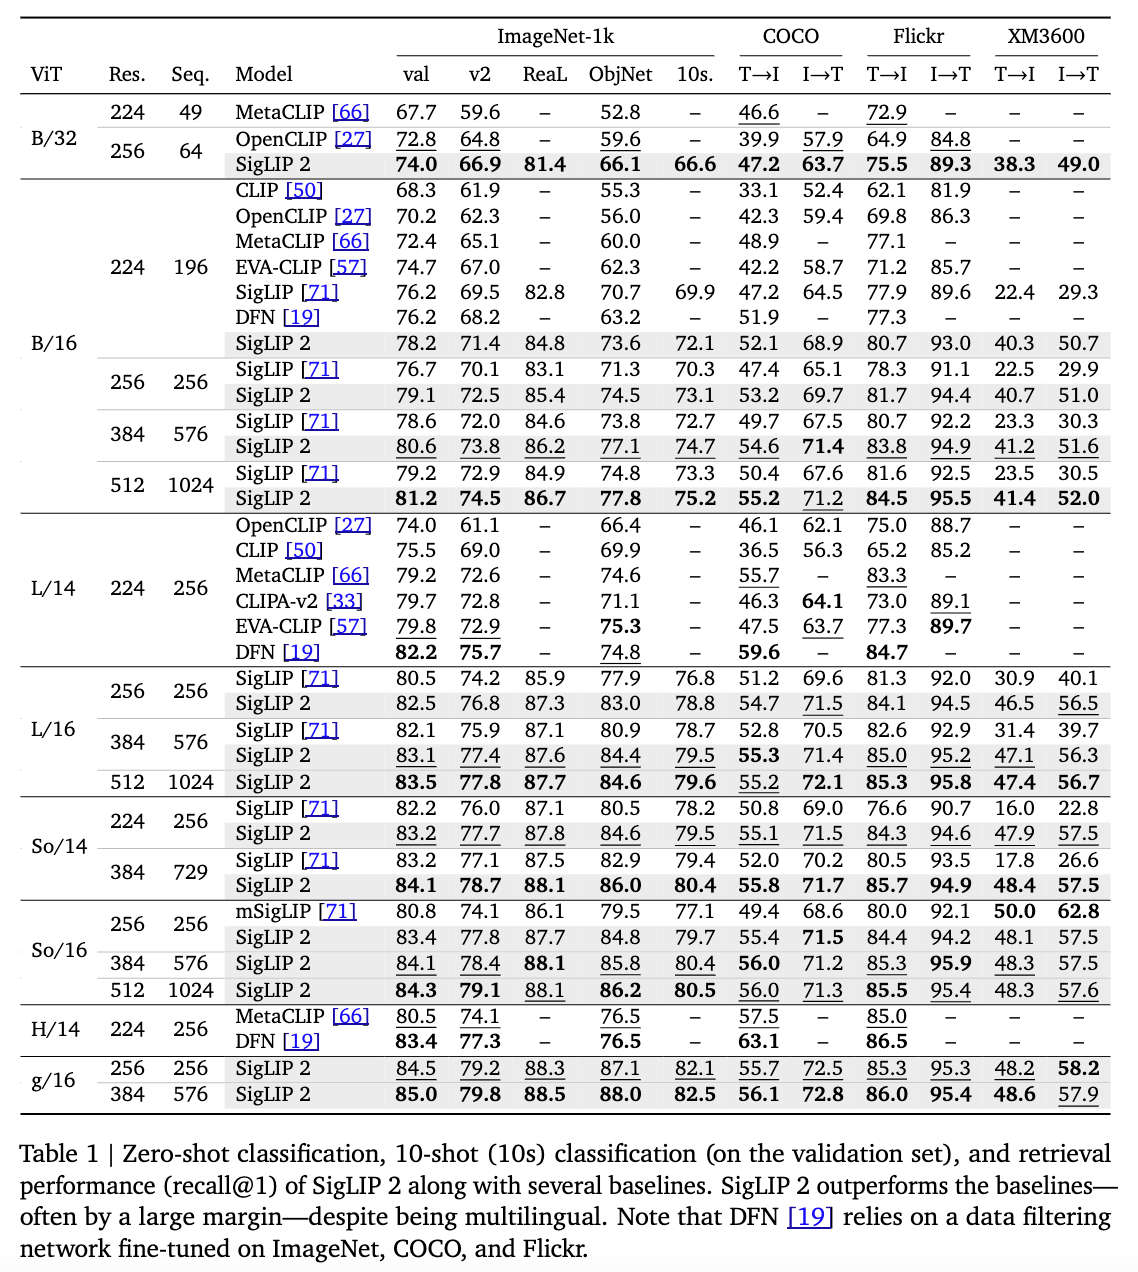
\includegraphics[width=\linewidth]{images/SigLIP2/fig-02.png}
\end{tcolorbox}
\end{tcbraster}
\par\vspace{0.95em}\noindent{\zihao{3}\bfseries \textcolor{feishuBlue}{3.2} SigLIP2作为vlm的视觉编码器}\par\vspace{0.28em}
\begin{tcbraster}[raster columns=2,raster equal height=rows,raster column skip=9pt,raster row skip=8pt,raster left skip=0pt,raster right skip=0pt]
\begin{tcolorbox}[blankest,valign=top]
视觉编码器如CLIP和SigLIP的一个常见用途是为VLMs提取视觉表示。通常的做法是将预训练的视觉编码器与预训练的LLM结合，并在丰富的视觉语言任务混合上进行多模态训练。\par
具体来说，将SigLIP 2视觉编码器和基准与Gemma2 2B LLM结合，并在包含字幕、OCR、定向字幕、视觉问答、检测和实例分割的Stage 1训练集上的5000万例子上训练LLM。我们保持视觉编码器冻结（这对质量几乎没有影响）并减少训练时间以反映典型的开放模型使用情况。生成的VLM随后在广泛的下游任务上进行微调，使用相关文献中的迁移设置。为了理解输入分辨率的影响，我们在分辨率224或256（对应于分别提取256个图像token的14和16的patch大小的模型）和384px上进行实验，但与相关文献不同的是，我们在384px上重复Stage 1，而不是从224px变体开始。\par
总体来看，SigLIP 2在各个分辨率和模型大小上明显优于SigLIP。对于L尺寸的视觉编码器，SigLIP 2也优于最近发布的AIMv2模型。\par
\end{tcolorbox}
\begin{tcolorbox}[blankest,valign=top]
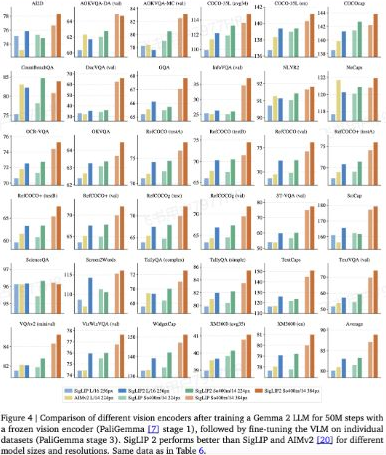
\includegraphics[width=\linewidth]{images/SigLIP2/fig-03.png}
\end{tcolorbox}
\end{tcbraster}
\end{document}
